\documentclass{standalone}
\usepackage{tikz}
\usetikzlibrary{patterns, positioning}


\begin{document}
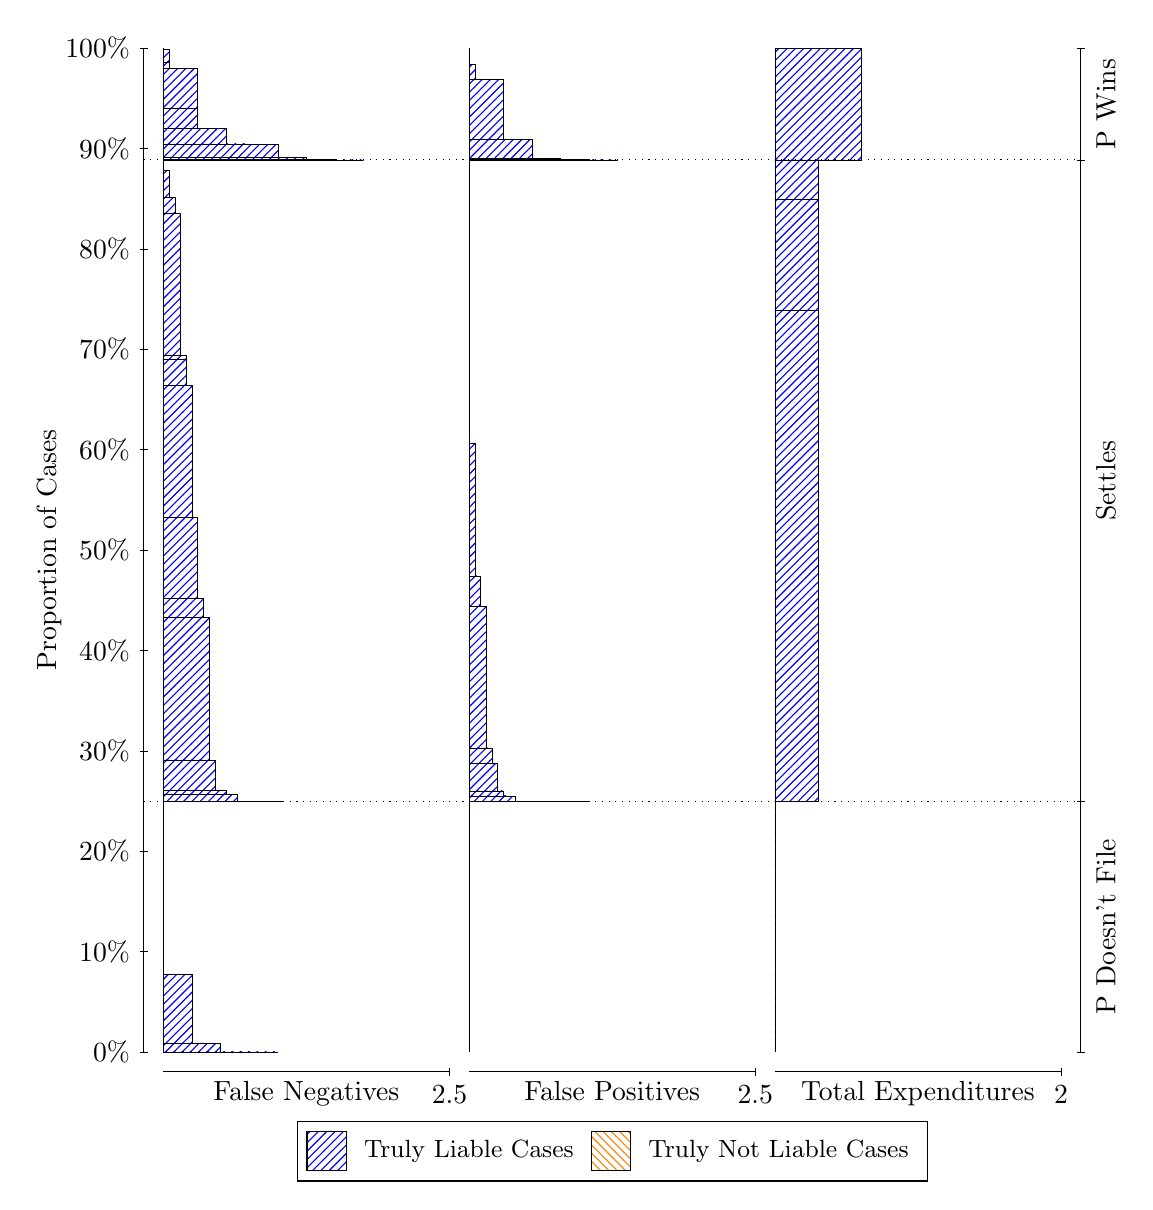
\begin{tikzpicture}
\draw[black, very thin] (1.5,1.75) -- (1.5,14.5);
\node[rotate=90, text=black, anchor=center] at (0.3, 8.125) {Proportion of Cases};
\draw[black, very thin] (1.45,1.75) -- (1.55,1.75);
\node[text=black, anchor=east] at (1.45, 1.75) {0\%};
\draw[black, very thin] (1.45,3.025) -- (1.55,3.025);
\node[text=black, anchor=east] at (1.45, 3.025) {10\%};
\draw[black, very thin] (1.45,4.3) -- (1.55,4.3);
\node[text=black, anchor=east] at (1.45, 4.3) {20\%};
\draw[black, very thin] (1.45,5.575) -- (1.55,5.575);
\node[text=black, anchor=east] at (1.45, 5.575) {30\%};
\draw[black, very thin] (1.45,6.85) -- (1.55,6.85);
\node[text=black, anchor=east] at (1.45, 6.85) {40\%};
\draw[black, very thin] (1.45,8.125) -- (1.55,8.125);
\node[text=black, anchor=east] at (1.45, 8.125) {50\%};
\draw[black, very thin] (1.45,9.4) -- (1.55,9.4);
\node[text=black, anchor=east] at (1.45, 9.4) {60\%};
\draw[black, very thin] (1.45,10.675) -- (1.55,10.675);
\node[text=black, anchor=east] at (1.45, 10.675) {70\%};
\draw[black, very thin] (1.45,11.95) -- (1.55,11.95);
\node[text=black, anchor=east] at (1.45, 11.95) {80\%};
\draw[black, very thin] (1.45,13.225) -- (1.55,13.225);
\node[text=black, anchor=east] at (1.45, 13.225) {90\%};
\draw[black, very thin] (1.45,14.5) -- (1.55,14.5);
\node[text=black, anchor=east] at (1.45, 14.5) {100\%};

\draw[black, very thin] (13.4,1.75) -- (13.4,14.5);
\draw[black, very thin] (13.35,1.75) -- (13.45,1.75);
\node[anchor=west] at (13.35, 1.75) {};
\draw[black, very thin] (13.35,4.9313) -- (13.45,4.9313);
\node[anchor=west] at (13.35, 4.9313) {};
\draw[black, very thin] (13.35,13.08) -- (13.45,13.08);
\node[anchor=west] at (13.35, 13.08) {};
\draw[black, very thin] (13.35,14.5) -- (13.45,14.5);
\node[anchor=west] at (13.35, 14.5) {};

\draw[black, very thin, pattern color=blue, pattern=north east lines] (1.75,1.75) rectangle (3.2033,1.75);
\draw[black, very thin, pattern color=blue, pattern=north east lines] (1.75,1.75) rectangle (2.84,1.7509);
\draw[black, very thin, pattern color=blue, pattern=north east lines] (1.75,1.7509) rectangle (2.4767,1.8624);
\draw[black, very thin, pattern color=blue, pattern=north east lines] (1.75,1.8624) rectangle (2.1133,2.7337);
\draw[black, very thin, pattern color=orange, pattern=north west lines] (1.75,2.7337) rectangle (1.75,2.7337);
\draw[black, very thin, pattern color=blue, pattern=north east lines] (1.75,2.7337) rectangle (1.75,4.9313);
\draw[black, very thin, pattern color=blue, pattern=north east lines] (1.75,4.9313) rectangle (3.276,4.9313);
\draw[black, very thin, pattern color=blue, pattern=north east lines] (1.75,4.9313) rectangle (3.1307,4.9313);
\draw[black, very thin, pattern color=blue, pattern=north east lines] (1.75,4.9313) rectangle (2.9853,4.9313);
\draw[black, very thin, pattern color=blue, pattern=north east lines] (1.75,4.9313) rectangle (2.9127,4.9313);
\draw[black, very thin, pattern color=blue, pattern=north east lines] (1.75,4.9313) rectangle (2.7673,4.9313);
\draw[black, very thin, pattern color=blue, pattern=north east lines] (1.75,4.9313) rectangle (2.6947,5.022);
\draw[black, very thin, pattern color=blue, pattern=north east lines] (1.75,5.022) rectangle (2.622,5.0241);
\draw[black, very thin, pattern color=blue, pattern=north east lines] (1.75,5.0241) rectangle (2.5493,5.0681);
\draw[black, very thin, pattern color=blue, pattern=north east lines] (1.75,5.0681) rectangle (2.404,5.4583);
\draw[black, very thin, pattern color=blue, pattern=north east lines] (1.75,5.4583) rectangle (2.404,5.4608);
\draw[black, very thin, pattern color=blue, pattern=north east lines] (1.75,5.4608) rectangle (2.3313,7.2653);
\draw[black, very thin, pattern color=blue, pattern=north east lines] (1.75,7.2653) rectangle (2.2587,7.5115);
\draw[black, very thin, pattern color=blue, pattern=north east lines] (1.75,7.5115) rectangle (2.186,8.5356);
\draw[black, very thin, pattern color=blue, pattern=north east lines] (1.75,8.5356) rectangle (2.1133,10.214);
\draw[black, very thin, pattern color=blue, pattern=north east lines] (1.75,10.214) rectangle (2.0407,10.552);
\draw[black, very thin, pattern color=blue, pattern=north east lines] (1.75,10.552) rectangle (2.0407,10.6);
\draw[black, very thin, pattern color=blue, pattern=north east lines] (1.75,10.6) rectangle (1.968,12.399);
\draw[black, very thin, pattern color=blue, pattern=north east lines] (1.75,12.399) rectangle (1.8953,12.602);
\draw[black, very thin, pattern color=blue, pattern=north east lines] (1.75,12.602) rectangle (1.8227,12.946);
\draw[black, very thin, pattern color=orange, pattern=north west lines] (1.75,12.946) rectangle (1.75,12.946);
\draw[black, very thin, pattern color=blue, pattern=north east lines] (1.75,12.946) rectangle (1.75,13.08);
\draw[black, very thin, pattern color=blue, pattern=north east lines] (1.75,13.08) rectangle (4.2933,13.08);
\draw[black, very thin, pattern color=blue, pattern=north east lines] (1.75,13.08) rectangle (3.93,13.081);
\draw[black, very thin, pattern color=blue, pattern=north east lines] (1.75,13.081) rectangle (3.5667,13.108);
\draw[black, very thin, pattern color=blue, pattern=north east lines] (1.75,13.108) rectangle (3.276,13.108);
\draw[black, very thin, pattern color=blue, pattern=north east lines] (1.75,13.108) rectangle (3.2033,13.272);
\draw[black, very thin, pattern color=blue, pattern=north east lines] (1.75,13.272) rectangle (2.9127,13.272);
\draw[black, very thin, pattern color=blue, pattern=north east lines] (1.75,13.272) rectangle (2.84,13.284);
\draw[black, very thin, pattern color=blue, pattern=north east lines] (1.75,13.284) rectangle (2.5493,13.479);
\draw[black, very thin, pattern color=blue, pattern=north east lines] (1.75,13.479) rectangle (2.4767,13.479);
\draw[black, very thin, pattern color=blue, pattern=north east lines] (1.75,13.479) rectangle (2.186,13.737);
\draw[black, very thin, pattern color=blue, pattern=north east lines] (1.75,13.737) rectangle (2.186,14.244);
\draw[black, very thin, pattern color=blue, pattern=north east lines] (1.75,14.244) rectangle (2.1133,14.244);
\draw[black, very thin, pattern color=blue, pattern=north east lines] (1.75,14.244) rectangle (1.8227,14.324);
\draw[black, very thin, pattern color=blue, pattern=north east lines] (1.75,14.324) rectangle (1.8227,14.484);
\draw[black, very thin, pattern color=orange, pattern=north west lines] (1.75,14.484) rectangle (1.75,14.484);
\draw[black, very thin, pattern color=blue, pattern=north east lines] (1.75,14.484) rectangle (1.75,14.5);
\draw[black, very thin, pattern color=orange, pattern=north west lines] (5.6333,1.75) rectangle (5.6333,1.75);
\draw[black, very thin, pattern color=blue, pattern=north east lines] (5.6333,1.75) rectangle (5.6333,4.9313);
\draw[black, very thin, pattern color=orange, pattern=north west lines] (5.6333,4.9313) rectangle (7.1593,4.9313);
\draw[black, very thin, pattern color=blue, pattern=north east lines] (5.6333,4.9313) rectangle (7.1593,4.9313);
\draw[black, very thin, pattern color=orange, pattern=north west lines] (5.6333,4.9313) rectangle (6.8687,4.9313);
\draw[black, very thin, pattern color=blue, pattern=north east lines] (5.6333,4.9313) rectangle (6.8687,4.9313);
\draw[black, very thin, pattern color=blue, pattern=north east lines] (5.6333,4.9313) rectangle (6.796,4.9313);
\draw[black, very thin, pattern color=orange, pattern=north west lines] (5.6333,4.9313) rectangle (6.578,4.9313);
\draw[black, very thin, pattern color=blue, pattern=north east lines] (5.6333,4.9313) rectangle (6.578,4.9313);
\draw[black, very thin, pattern color=blue, pattern=north east lines] (5.6333,4.9313) rectangle (6.5053,4.9313);
\draw[black, very thin, pattern color=blue, pattern=north east lines] (5.6333,4.9313) rectangle (6.4327,4.9313);
\draw[black, very thin, pattern color=orange, pattern=north west lines] (5.6333,4.9313) rectangle (6.2873,4.9313);
\draw[black, very thin, pattern color=blue, pattern=north east lines] (5.6333,4.9313) rectangle (6.2873,4.9319);
\draw[black, very thin, pattern color=blue, pattern=north east lines] (5.6333,4.9319) rectangle (6.2147,4.9962);
\draw[black, very thin, pattern color=orange, pattern=north west lines] (5.6333,4.9962) rectangle (6.142,4.9962);
\draw[black, very thin, pattern color=blue, pattern=north east lines] (5.6333,4.9962) rectangle (6.142,5.0026);
\draw[black, very thin, pattern color=blue, pattern=north east lines] (5.6333,5.0026) rectangle (6.0693,5.0659);
\draw[black, very thin, pattern color=orange, pattern=north west lines] (5.6333,5.0659) rectangle (5.9967,5.0659);
\draw[black, very thin, pattern color=blue, pattern=north east lines] (5.6333,5.0659) rectangle (5.9967,5.4102);
\draw[black, very thin, pattern color=blue, pattern=north east lines] (5.6333,5.4102) rectangle (5.924,5.6125);
\draw[black, very thin, pattern color=blue, pattern=north east lines] (5.6333,5.6125) rectangle (5.8513,7.4122);
\draw[black, very thin, pattern color=blue, pattern=north east lines] (5.6333,7.4122) rectangle (5.7787,7.7972);
\draw[black, very thin, pattern color=blue, pattern=north east lines] (5.6333,7.7972) rectangle (5.706,9.4761);
\draw[black, very thin, pattern color=blue, pattern=north east lines] (5.6333,9.4761) rectangle (5.6333,13.08);
\draw[black, very thin, pattern color=orange, pattern=north west lines] (5.6333,13.08) rectangle (7.5227,13.08);
\draw[black, very thin, pattern color=blue, pattern=north east lines] (5.6333,13.08) rectangle (7.5227,13.08);
\draw[black, very thin, pattern color=orange, pattern=north west lines] (5.6333,13.08) rectangle (7.1593,13.08);
\draw[black, very thin, pattern color=blue, pattern=north east lines] (5.6333,13.08) rectangle (7.1593,13.081);
\draw[black, very thin, pattern color=orange, pattern=north west lines] (5.6333,13.081) rectangle (6.796,13.081);
\draw[black, very thin, pattern color=blue, pattern=north east lines] (5.6333,13.081) rectangle (6.796,13.096);
\draw[black, very thin, pattern color=orange, pattern=north west lines] (5.6333,13.096) rectangle (6.4327,13.096);
\draw[black, very thin, pattern color=blue, pattern=north east lines] (5.6333,13.096) rectangle (6.4327,13.337);
\draw[black, very thin, pattern color=orange, pattern=north west lines] (5.6333,13.337) rectangle (6.142,13.337);
\draw[black, very thin, pattern color=blue, pattern=north east lines] (5.6333,13.337) rectangle (6.142,13.337);
\draw[black, very thin, pattern color=blue, pattern=north east lines] (5.6333,13.337) rectangle (6.0693,14.102);
\draw[black, very thin, pattern color=orange, pattern=north west lines] (5.6333,14.102) rectangle (5.7787,14.102);
\draw[black, very thin, pattern color=blue, pattern=north east lines] (5.6333,14.102) rectangle (5.7787,14.102);
\draw[black, very thin, pattern color=blue, pattern=north east lines] (5.6333,14.102) rectangle (5.706,14.296);
\draw[black, very thin, pattern color=orange, pattern=north west lines] (5.6333,14.296) rectangle (5.6333,14.296);
\draw[black, very thin, pattern color=blue, pattern=north east lines] (5.6333,14.296) rectangle (5.6333,14.5);
\draw[black, very thin, pattern color=orange, pattern=north west lines] (9.5167,1.75) rectangle (9.5167,1.75);
\draw[black, very thin, pattern color=blue, pattern=north east lines] (9.5167,1.75) rectangle (9.5167,4.9313);
\draw[black, very thin, pattern color=orange, pattern=north west lines] (9.5167,4.9313) rectangle (10.062,4.9313);
\draw[black, very thin, pattern color=blue, pattern=north east lines] (9.5167,4.9313) rectangle (10.062,11.164);
\draw[black, very thin, pattern color=orange, pattern=north west lines] (9.5167,11.164) rectangle (10.062,11.164);
\draw[black, very thin, pattern color=blue, pattern=north east lines] (9.5167,11.164) rectangle (10.062,12.576);
\draw[black, very thin, pattern color=orange, pattern=north west lines] (9.5167,12.576) rectangle (10.062,12.576);
\draw[black, very thin, pattern color=blue, pattern=north east lines] (9.5167,12.576) rectangle (10.062,13.08);
\draw[black, very thin, pattern color=orange, pattern=north west lines] (9.5167,13.08) rectangle (10.607,13.08);
\draw[black, very thin, pattern color=blue, pattern=north east lines] (9.5167,13.08) rectangle (10.607,14.5);
\draw[black, dotted] (1.5,4.9313) -- (13.4,4.9313);
\draw[black, dotted] (1.5,13.08) -- (13.4,13.08);
\draw[black, very thin] (1.75,1.5) -- (5.3833,1.5);
\node[text=black, anchor=north] at (3.5667, 1.5) {False Negatives};
\draw[black, very thin] (5.3833,1.45) -- (5.3833,1.55);
\node[text=black, anchor=north] at (5.3833, 1.45) {2.5};

\draw[black, very thin] (5.6333,1.5) -- (9.2667,1.5);
\node[text=black, anchor=north] at (7.45, 1.5) {False Positives};
\draw[black, very thin] (9.2667,1.45) -- (9.2667,1.55);
\node[text=black, anchor=north] at (9.2667, 1.45) {2.5};

\draw[black, very thin] (9.5167,1.5) -- (13.15,1.5);
\node[text=black, anchor=north] at (11.333, 1.5) {Total Expenditures};
\draw[black, very thin] (13.15,1.45) -- (13.15,1.55);
\node[text=black, anchor=north] at (13.15, 1.45) {2};

\node[text=black, centered, rotate=90] at (13.72, 3.3406) {P Doesn't File};
\node[text=black, centered, rotate=90] at (13.72, 9.0059) {Settles};
\node[text=black, centered, rotate=90] at (13.72, 13.79) {P Wins};

\draw (7.449999999999999,1.5) node[draw=none] (baseCoordinate) {};
\begin{scope}[align=center]
        \matrix[scale=0.5, draw=black, below=0.5cm of baseCoordinate, nodes={draw}, column sep=0.1cm]{
            \node[rectangle, draw, minimum width=0.5cm, minimum height=0.5cm, pattern color=blue, pattern=north east lines] {}; &
            \node[draw=none, font=\small, text=black] (B) {Truly Liable Cases}; &
            \node[rectangle, draw, minimum width=0.5cm, minimum height=0.5cm, pattern color=orange, pattern=north west lines] {}; &
            \node[draw=none, font=\small, text=black] (B) {Truly Not Liable Cases}; \\
            };
\end{scope}

\end{tikzpicture}
\end{document}